\documentclass[11pt]{article}
\usepackage[margin=0.75in]{geometry}
\usepackage{amsmath}
\usepackage{tikz}
\usepackage{enumitem}
\usepackage{siunitx}
\setlength{\parindent}{0pt}
\newcommand{\graphbox}{\begin{center}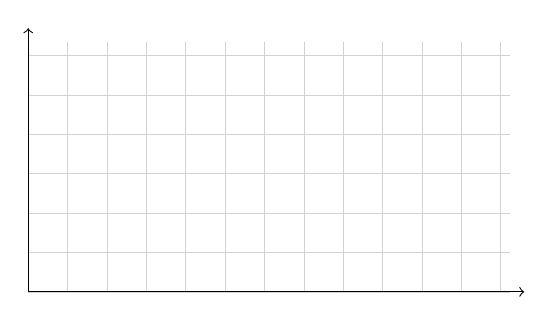
\begin{tikzpicture}[x=0.72cm,y=0.72cm]
\draw[step=0.5cm,gray!35,very thin] (0,0) grid (8.5,4.4);
\draw[->] (0,0)--(8.75,0);
\draw[->] (0,0)--(0,4.65);
\end{tikzpicture}\end{center}}
\begin{document}
\begin{center}\Large\textbf{AP Physics 1 1D Motion Post-Lab Quiz -- Version A}\end{center}
\vspace{0.08in}\textbf{Name:} \rule{2.1in}{0.4pt}\hfill\textbf{Period:} \rule{0.65in}{0.4pt}\hfill\textbf{Date:} \rule{1.1in}{0.4pt}
\vspace{0.12in}
\begin{enumerate}[leftmargin=*,itemsep=0.15in]
\item A student releases a ball from rest from a fixed height above the floor. The student wants to determine whether the ball's downward acceleration remains approximately constant while it falls. The available equipment is a ball, a meterstick, a stopwatch, tape, and enough vertical space for a safe drop.

\textbf{a.} Describe the measurements the student should collect during the fall.\\
\textbf{b.} Describe how the student could analyze those measurements to determine whether the acceleration is approximately constant.
\vspace{0.55in}

\item A student records a ball falling vertically. At first, the student places several individual tape marks next to the path of the ball. The student then replaces the tape marks with a meterstick positioned vertically next to the entire path of the fall.

\textbf{a.} Explain how using the meterstick could make the position measurements easier to collect.\\
\textbf{b.} Explain one way this change could make the measurements more consistent.
\vspace{0.55in}

\item A student releases a ball from rest and records its distance fallen at several times.

\begin{center}
\begin{tabular}{c|cccccc}
Time $t$ (s) & 0.00 & 0.10 & 0.20 & 0.30 & 0.40 & 0.50\\ \hline
Distance fallen $d$ (m) & 0.000 & 0.048 & 0.197 & 0.440 & 0.786 & 1.228
\end{tabular}
\end{center}
\textbf{a.} Transform the data as needed to produce a linear graph. Using the graph space provided, plot the appropriate variables, clearly label both axes with units, and draw a best-fit line.\\
\textbf{b.} Describe the shape of your graph. Based on the graph, determine whether the ball's acceleration was approximately constant and explain your reasoning.

\graphbox
\end{enumerate}
\end{document}
